\section{Capacitor Characteristics}
\subsection{Capacitance}
An ideal capacitor only has a value of capacitance, which is defined as the ablity to store an electrcial charge. 

The equation for a parallel plate capacitor is:

$C = \epsilon _0\epsilon A/d$

"
$\epsilon _0$ is the permitivity of free space and has a value of $8.85 * 10^{-11} F/m$

$\epsilon$ is the permitivity of the dielectric

$A$ is the area of the plates

$d$ is the distance between the plates (i.e. the thickness of the dielectric)
"

In the case of an ideal capacitor, it only has the property of capacitance (no inductance or resistance), and does not vary over frequency, voltage, or temperature.  \cite{disc_comp}

Why do I care about this property?

In using a capacitors for bypassing, you want to eliminate signals above the highest frequency of interest (noise). In doing this, you want to choose a capacitor who's capacitance is low (<1 Ohm), in order to shunt the high frequencies to ground. For an ideal capacitor, you would just choose a large value capacitance and call it a day. Practical parameters (parasitics), make this not so good of a strategy. 

In using a capacitor for filtering (such as a single pole low pass filter) you set the cut off of the filter via (1/2*pi*rc) to filter out the frequencies of interest, while passing the frequencies that you desire. 

\subsection{ESR}

Equivalent series resistance is the resistance measured between the leads and the capcitor plate?? It is most important when there are high AC currents flowing, as they will dissipate power through the ESR. 
\cite{anal_capProps}

Good:
\begin{itemize}
    \item Mica
    \item film
    \cite{anal_capProps}
\end{itemize}

---

ESR is the sum of all of the resistive components of the capacitor. It is typically modeled as a "single series resistance with the capacitance."

We care about high ESR with:
high AC currents
RF
high ripple currents

We don't care about high ESR with:
"Precision, high impedance, low level analog circuits"
\cite[Sect.~3.6.7]{elec_inv}

low esr:
mica
film

Knowing the ESR of a capacitor allows you to know how much power will be dissipated in it when it is filtering a switching power supply.\cite[Sect.~3.6.7]{elec_inv}

---

Even though ESR is measured in units of ohms and seen as a resistance, it is not the same at all frequencies. Therefore, it is typically given at a particular frequency.

electrolytic bypass -- 120Hz
tantalums used switchers -- 100kHz

eletrolytics -- higher at low frequencies
\cite{capSite_intro}

\subsection{ESL}

Equivalent series inductance is the inductance seen looking into one of the leads of the capcitor. It causes the most problems at high frequencies, where it can dominate the capacitve component of the capacitor. 
\cite{anal_capProps}

Good:
MLCC

Bad:
\begin{itemize}
    \item electrolytic
    \item paper
    \item plastic film\cite{anal_capProps}
\end{itemize}

---

ESL is primarily composed of the capictor's leads that are in series with the capacitive portion of the capacitor. It is modeled as an inductor in series with C. ESL is the main reason for why you need at least 2 capacitors to decouple your power supply. As frequency increases past the point where $X_c == X_{ESL}$, the capacitor's impedance begins to increase with frquency, making it quite useless as a bypass element. 

bad:
\begin{itemize}
    \item electrolytic
    \item paper
    \item plastic-film
\end{itemize}

good:
\begin{itemize}
    \item mica
    \item MLCC
\end{itemize}

Some MLCCs can be self-resonant with a high Q b/c of low ESR.
\cite[Sect.~3.6.7]{elec_inv}

\subsection{Dissipation Factor}

The dissipation factor of a capacitor is the "ratio of the energy dissipated per cycle to energy stored per cycle." It is a paramater which lumps together the effects of ESR and ESL. DF = power factor ($cos(\phi)$). $DF = 1 / Q.$
\cite{anal_capProps}

---

"The ratio of energy dissipated per cycle to energy stored per cycle." "It is also the ratio of the current in phase with teh applied voltage to the reactive current."

D = 1/Q

A capacitor with a lower D is a more efficient component.
\cite[Sect.~3.6.7]{elec_inv}

----

We are particularely concerned about DF when dealing with applications concerning AC or high ripple currents.

$DF = ESR / X_c$

DF is comprised of:
\begin{enumerate}
    \item Metal losses
    \begin{enumerate}
        \item Resistance of leads
        \item Resistance of end terminations
        \item Resistance of metal foil or film
    \end{enumerate}
    \item insulation resistance (small)
    \item dielectric losses
\end{enumerate}
\cite{capSite_intro}

\begin{figure}
    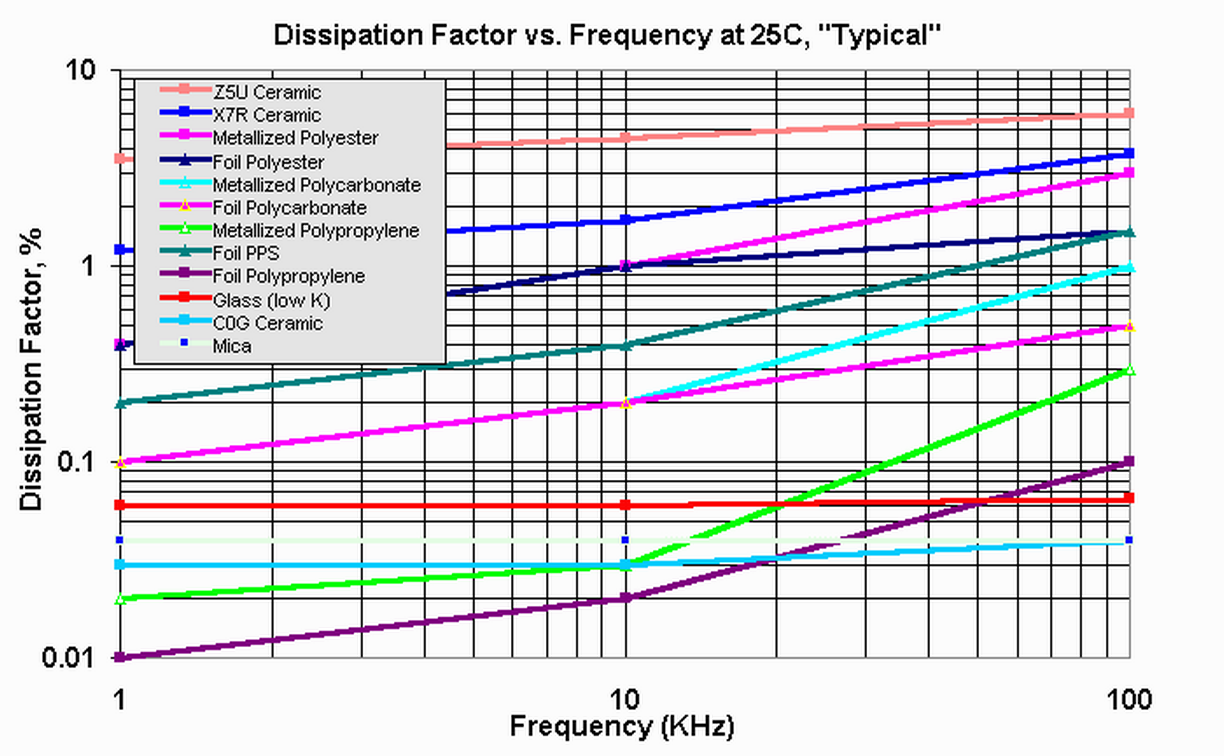
\includegraphics[keepaspectratio=true,scale=0.25]{../figures/df_vs_freq.png}
    \centering
    \cite{capSite_df_vs_freq}
    \caption{Dissipation Factor vs Frequency}
    \label{df_vs_freq}
\end{figure}

\begin{figure}
    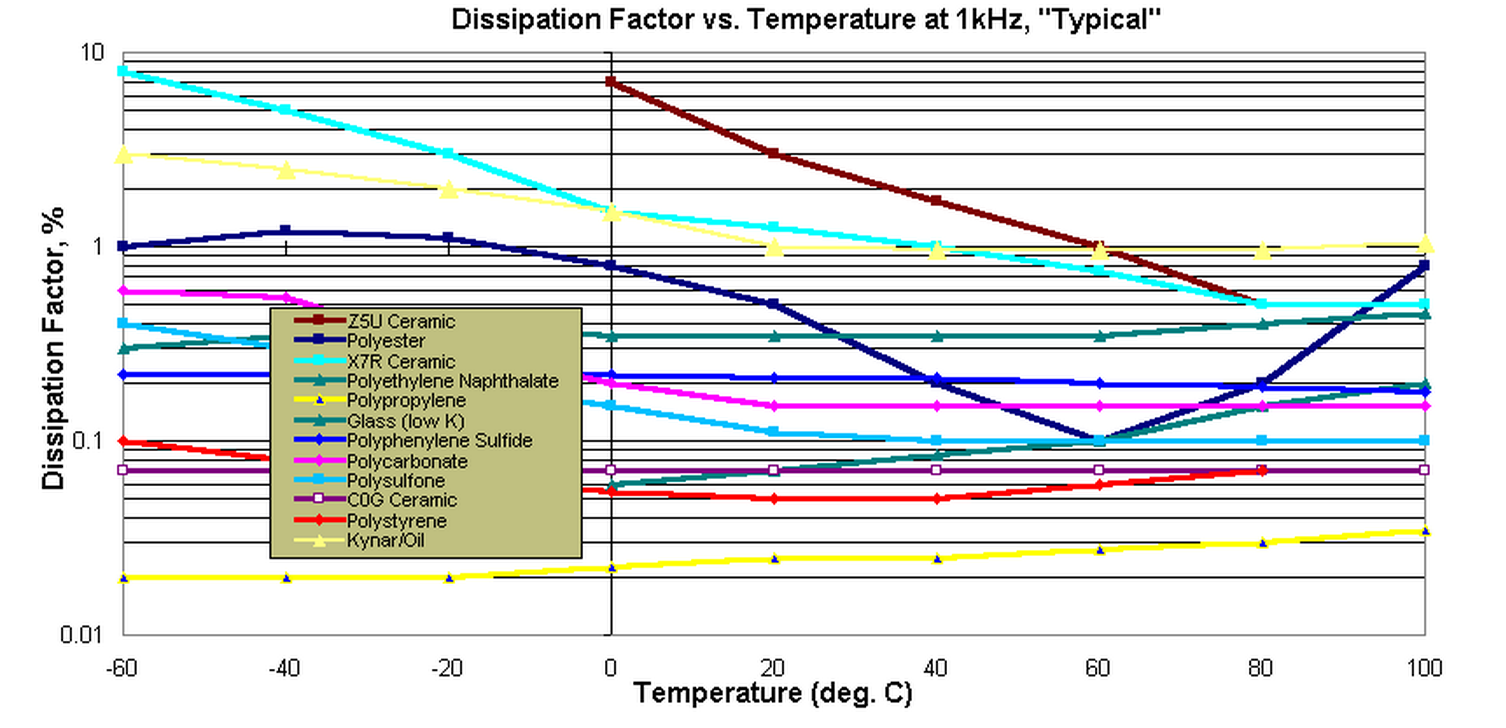
\includegraphics[keepaspectratio=true,scale=0.2]{../figures/df_vs_temp.png}
    \centering
    \cite{capSite_df_vs_temp}
    \caption{Dissipation Factor vs Temperature}
    \label{df_vs_temp}
\end{figure}



\subsection{List}
\cite{leon_cap}
\begin{enumerate}
    \item ESR
    \item ESL
    \item Leakage Current
    \item Dielectric Absorption
    \item Quality Factor
    \item Dissipation factor (or dielectric loss)
    \item Loss Tangent
    \item Self Resonant Frequency
    \item Capacitance stability with time
    \item Capacitance stability with temperature
    \item Capacitance stability with applied valtage
    \item High-frequency properties and effects
    \item Voltage rating and dielectric strength
    \item Insulation resistance
    \item Isolation resistance
    \item Insulation resistance variations with temperature
    \item Pulse operation and surge rating
    \item Effects of radiation
    \item Effects of vibrariton and shock
\end{enumerate}

"With many types of capacitors, further derating is required as the operating frequency increases."\cite[Sect.~3.6.7]{elec_inv}

\subsection {Models}
The ideal capacitor model will only bring you so far before you need to graduate to a more complex understanding. The industry typically calls any paramaters beyond the basic capcitor model "parasitic effects," because they typically degrade the performance of a capcitor from the ideal. Nonetheless, they are present in every capcitor to varying degrees. It is imparative to know which models to use in which circumstances. 

\begin{figure}
    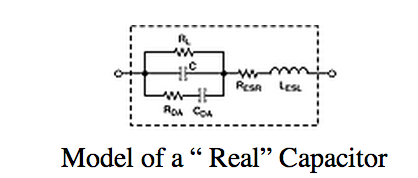
\includegraphics[keepaspectratio=true,scale=0.75]{../figures/completeModel.png}
    \centering
    \cite{anal_capProps}
    \caption{Complete Model}
    \label{completeModel}
\end{figure}

\begin{figure}
    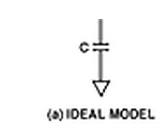
\includegraphics[keepaspectratio=true,scale=0.5]{../figures/idealModel.png}
    \centering
    \cite{anal_capProps}
    \caption{Ideal Model}
    \label{idealModel}
\end{figure}

\begin{figure}
    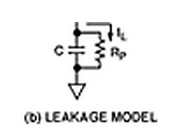
\includegraphics[keepaspectratio=true]{../figures/leakageModel.png}
    \centering
    \cite{anal_capProps}
    \caption{Leakage Model}
    \label{leakModel}
\end{figure}

\begin{figure}
    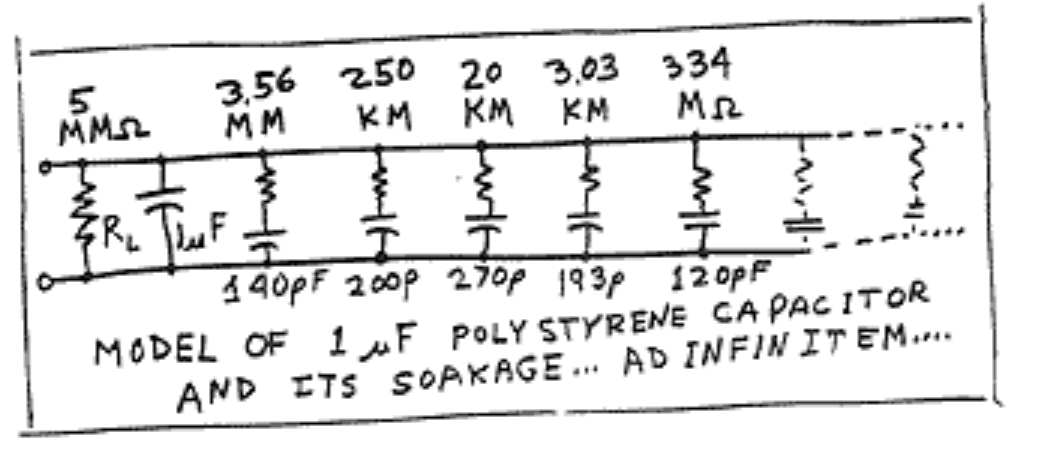
\includegraphics[keepaspectratio=true,scale=.3]{../figures/da_model.png}
    \centering
    \cite{rap_da}
    \caption{Dielectric Absorption Model}
    \label{daModel}
\end{figure}

\begin{figure}
    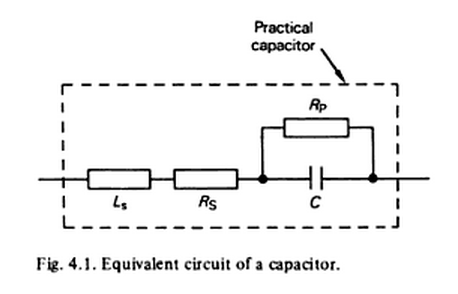
\includegraphics[keepaspectratio=true,scale=.7]{../figures/capModel_discComp.png}
    \centering
    \cite{disc_comp}
    \caption{Practical Model}
    \label{pracModel}
\end{figure}

\subsection{Voltage Dependence}

"Materials with high permitivity tend to have characteristics which are voltage dependent."\cite{disc_comp}

\subsection{Equivalent Circuits}
\subsubsection{Ls, Rs, C, \& Rp}

Refer to Figure: \ref{fig:pracModel} for this section.

"

$R_P$ is the leakage or insulation resistance

$R_S$ is the series resistance

ESR is the ac resistance and incorporate both $R_P$ and $R_S$.

$L_S$ is the self inductance 

$Z = (R_S^2 + X_C^2)^{1/2}$

$cos(\phi) = R_S / Z$

$tan(\delta) = R_S / X_C$

where:

$Z$ is the impedance of the capacitor

$X_C = 1 / 2\pi fC$ and is the capacitor reactance at frequency f.

$cos(\phi)$ is the power factor

$tan(\delta)$ is the loss angle, loss tangent, or dissipation factor of the capacitor.

"

\cite{disc_comp}

Power factor varies with temperature, but plummets below 0DegC.
Dissipation factor is sensitive to moisture.\cite{disc_comp}

\subsection{Voltage Dependence}

"Materials with high permitivity tend to have characteristics which are voltage dependent."\cite{disc_comp}

\subsection{Equivalent Circuits}
\subsubsection{Ls, Rs, C, \& Rp}

Refer to Figure: \ref{fig:pracModel} for this section.

"

$R_P$ is the leakage or insulation resistance

$R_S$ is the series resistance

ESR is the ac resistance and incorporate both $R_P$ and $R_S$.

$L_S$ is the self inductance 

$Z = (R_S^2 + X_C^2)^{1/2}$

$cos(\phi) = R_S / Z$

$tan(\delta) = R_S / X_C$

where:

$Z$ is the impedance of the capacitor

$X_C = 1 / 2\pi fC$ and is the capacitor reactance at frequency f.

$cos(\phi)$ is the power factor

$tan(\delta)$ is the loss angle, loss tangent, or dissipation factor of the capacitor.

"

\cite{disc_comp}

Power factor varies with temperature, but plummets below 0DegC.
Dissipation factor is sensitive to moisture.\cite{disc_comp}


\subsection{Leakage}

As opposed to the ideal capcitor, which can hold its charge indefinitely, real capcitors have a leakage component. Over time, this parallel resistance bleeds aways the charge stored on the capcitor. This will happen with a time constant of C*R\_l. This parameter is especially important in circuits such as sample and hold applications.
\cite{anal_capProps}

Good:
\begin{itemize}
    \item teflon
    \item poly*
    \cite{anal_capProps}
    \item film 
    \begin{itemize}
        \item polypropylene 
        \item polystyrene \cite[Sect.~3.6.7]{elec_inv}
    \end{itemize}
\end{itemize}
\cite{capSite_intro}

Bad:
\begin{itemize}
    \item Electrolytic
    \item Aluminum
    \item Tantalum
    \cite{anal_capProps}
    \cite[Sect.~3.6.7]{elec_inv}
\end{itemize}

---

Certain capacitors can leak at rates of only 2.7mV/day. $\tau$ = 10 years. -- rap??

---

A charged capacitor will discharge with a time constant of C*RL. \cite[Sect.~3.6.7]{elec_inv}
This is assuming that there is no external volatge source, at which you would leak at V / (RL + ESR) ??? maybe?

---

aka Insualtion resistance (low leakage)
aka leakage current (high leakage)

Bad:
Electrolytics (worst)

Good

\begin{itemize}
    \item Film ($IR 1/\alpha \epsilon$)    
    \item COG ceramics
\end{itemize}

\subsection{Quality Factor}

$Q = 1/D$

$Q = X_c / R_{ESR}$

"Ratio of the energy stored to that dissipated per cycle." It is the capacitor's ability to store charge. It can also be thought of as an efficiency measurement. 

"The rate of heat conversion is generally in proportino to the power and frequency of the applied energy. Energy entering the dielectric, however, is attenuated at a rate proportional to the frueqnecy of teh elcetric field and the loss tangent of the material."
\cite[Sect.~3.6.7]{elec_inv}

\subsection{Space Charge}

"Space charge is charge in the dielectric, electrons, protons, nad ions, that is moved around by the applied voltage." Charge will build build up in the capacitor over time. They electrons are not able to return to their holes quickly due to the high dielectric resistance.


\cite[Space Charge]{capSite_intro}

\subsection{Dielectric Absorption}

Dielectric absorption is the name of the phenomenon that happens when a charged capcitor is quickly discharged and then left in the "open" state. After a certain amount of time, the voltage can restablish itself on the capacitor through charge that was trapped inside. This is why certain large value capacitors are shipped with a resistor acress their terminals. This burn resistor dissipates any voltage that would build up across the terminals of the capitor through.

Good:
poly*

Bad:
MLCC

---

Also known as dielectric soakage. Dielectric absorption (DA) is the ability of capacitors to recover a portion of their voltage when they are charged up and then rapidly discharged for a short amount of time. This effect can be dangerous, as a "discharged" capacitor can recover enough voltage to shock you.\cite{rap_da}

"This was well known in as early as the 1700s." \cite{rap_da}
1900s - said that DA was caused by molecules being polarized and then loosing their polarization when the applied voltage was removed.
DA also affects charging of capacitors. If you charge a capacitor to its working voltage, it will continue to need charge for some time after stabalizing at a voltage. Also DA is "fairly" linear.

The model for DA in a capacitor is C in parallel with R in parallel with a series of series RC sections. One should not forget about leakage when thinking about DA.

Polypropylne capacitors have low DA.

---

DA is commonly seen as a problem in long period integrators. \cite{rap_da2}

---

"At high frequencies, this means that the capacitor cannot complete its discharge, and this has the same effect as a loss in capacitance."\cite{disc_comp}

---

DA has hysteresis like properties.

"Dielectric absorption is a hysteresis-like internal charge distribution within the dielectric that causes a capacitor that is quickly discharged and then open-circuited to appear to recover some of its charge."

"charge memory effect that will cause errors in sample and hold circuits"

bad:
MLCC

DA = \% of charge stored in the dielectric. The rest of the charge is stored on the plates

DA = $V_{self-charge} / V_{before-discharge}$, with defined charge and discharge values or ratios.
\cite[Sect.~3.6.7]{elec_inv}

----

"DA aka 'soakage' 'voltge retention' 'return voltage'

In the model in Figure:\ref{fig:daModel}, we see that the parallel RC branches typically consist of high valued resistors with capacitors which are of lower values than the main C.

MIL-C-19978D -- 5min/5sec/1min sequence of charge, discharge, wait, and then measure.

good:
teflon
polystyrene
polypropylene

bad:
electrolytics
high-k ceramics
oil-filled

Typically, capacitors which have a high insulation resistance and a low $\mu$ have much better DA characteristics.

"However, while the RC model is usefull for predicting how DA will behave, it does not reflect the underlying physics."
\cite{capSite_intro}

\subsection{Insulation Resistance}
"This is a measure of the resistance to a dc current flow through the capacitor under steady-state conditions."\cite[Sect.~3.6.7]{elec_inv}
